\documentclass[10pt,journal,a4paper]{IEEEtran}
\usepackage[T1]{fontenc}
\usepackage{graphicx}
\usepackage{booktabs}
\usepackage{amsmath}
\usepackage{amssymb}
\usepackage{url}
\urlstyle{same}
\usepackage[hidelinks]{hyperref}

\begin{document}

\title{\vspace{-1.6em}\footnotesize\textsc{The University of Lahore $\bullet$ Department of Intelligent Systems $\bullet$ AI-101}\\[0.9em]
\Large Task C3: Image Captioning on Flickr8k}

\author{\normalsize Manaal Pervaiz \quad$\vert$\quad Roll No. 70173809 \quad$\vert$\quad Section BSES A\\
\normalsize Repository: \url{https://github.com/manaal6/AI101-ML-Assignment-70173809}\\
\normalsize Instructor: Dr. Muhammad Awais, AI Architect}
\date{}
\maketitle

\section{Introduction}
Image captioning turns a photograph into a sentence, requiring object, attribute,
count and action recognition plus fluent English. A convolutional encoder
summarises the image and a recurrent decoder generates words. We train this
encoder--decoder on Flickr8k with two frozen backbones and three decoders.
ResNet-50 with beam width 5 reaches corpus BLEU-4 21.64 on 1,091 test images;
beam search adds about two points over greedy decoding, and the two backbones
finish within 0.17 BLEU-4 of each other.

\section{Problem Statement}
Given an image $I$ and vocabulary $V$, predict $y=(y_1,\dots,y_T)$ describing
$I$. Training maximises $\sum_t \log p(y_t \mid y_{<t}, I)$ over five human
references. Evaluation uses corpus BLEU-1 to BLEU-4, distinct words and decoding
cost. Many captions are valid, so BLEU measures n-gram overlap rather than truth
and must be read with examples.

\section{Dataset Used}
Flickr8k \cite{hodosh} contains 8,091 Flickr photographs with five independent
captions each, 40,455 in total. We use the Kaggle mirror
\texttt{adityajn105/flickr8k} (\texttt{Images/} and \texttt{captions.txt}).
Captions are lower-cased, HTML-unescaped and stripped of punctuation and digits.
Splits are by image with seed 42 (6,000 train, 1,000 validation, 1,091 test), so
no image crosses splits. The vocabulary keeps words seen at least five times,
shrinking 7,439 types to 2,557; sequences are padded to 22 tokens and 3.24\% of
test tokens are unknown.

\section{Dataset Statistics}
Table~\ref{tab:data} summarises the corpus. Captions average 10.83 words
(median 10), so 22 tokens covers the tail. Five references stabilise corpus
BLEU, but Flickr8k is clean and centred, so these scores overstate in-the-wild
performance. The references also disagree in wording: eight test captions match
one reference exactly yet score far below 100 against all five.

\section{Methodology}
\subsection{Learning Setting}
The encoders are frozen ImageNet classifiers: ResNet-50 \cite{resnet}, whose
pooled output is 2,048-dimensional, and EfficientNet-B0 \cite{effnet}, which
gives 1,280 dimensions. Images are resized to 256, centre-cropped to 224 and
normalised with ImageNet statistics; features are cached once (118.9\,s and
59.5\,s on the T4). The decoder is a merge model: the image vector is projected
to 512 units (ReLU, dropout 0.3) and concatenated at every step with a 256-d
word embedding; a 512-unit LSTM predicts the next token. The models have 5.64M
and 5.25M parameters.

\subsection{Data Split Approach}
Splitting by image prevents near-duplicate photographs leaking across splits.
All five captions of a training image are separate examples (30,000 sequences),
and the vocabulary is built on training captions only. Validation selects the
early-stopping checkpoint; test is decoded once per configuration.

\subsection{Training and Decoding Settings}
Both decoders use Adam ($10^{-3}$, weight decay $10^{-5}$), batch 128, dropout
0.3 and padding-ignored cross-entropy, for at most 20 epochs with patience 3.
ResNet-50 stopped at epoch 16 (validation loss 2.6863), EfficientNet-B0 at 12
(2.7151). We decode greedily and with beam $k=3$ and $k=5$, scored by cumulative
log-probability without length normalisation. BLEU uses sacreBLEU \cite{sacrebleu}
over all five references.


\section{Results and Analysis}
\subsection{Results}
Table~\ref{tab:bleu} reports test BLEU, distinct words, mean length and decoding
time. The best BLEU-4 is 21.64 (ResNet-50, beam $k=5$); EfficientNet-B0 reaches
21.47, within the variation between beam widths. Beam search is decisive:
ResNet-50 rises from 19.51 (greedy) to 21.27 ($k=3$) and 21.64 ($k=5$). BLEU-2
and BLEU-3 follow the same order (41.97 to 45.07 and 28.97 to 31.72).


\begin{figure*}[t]
\centering
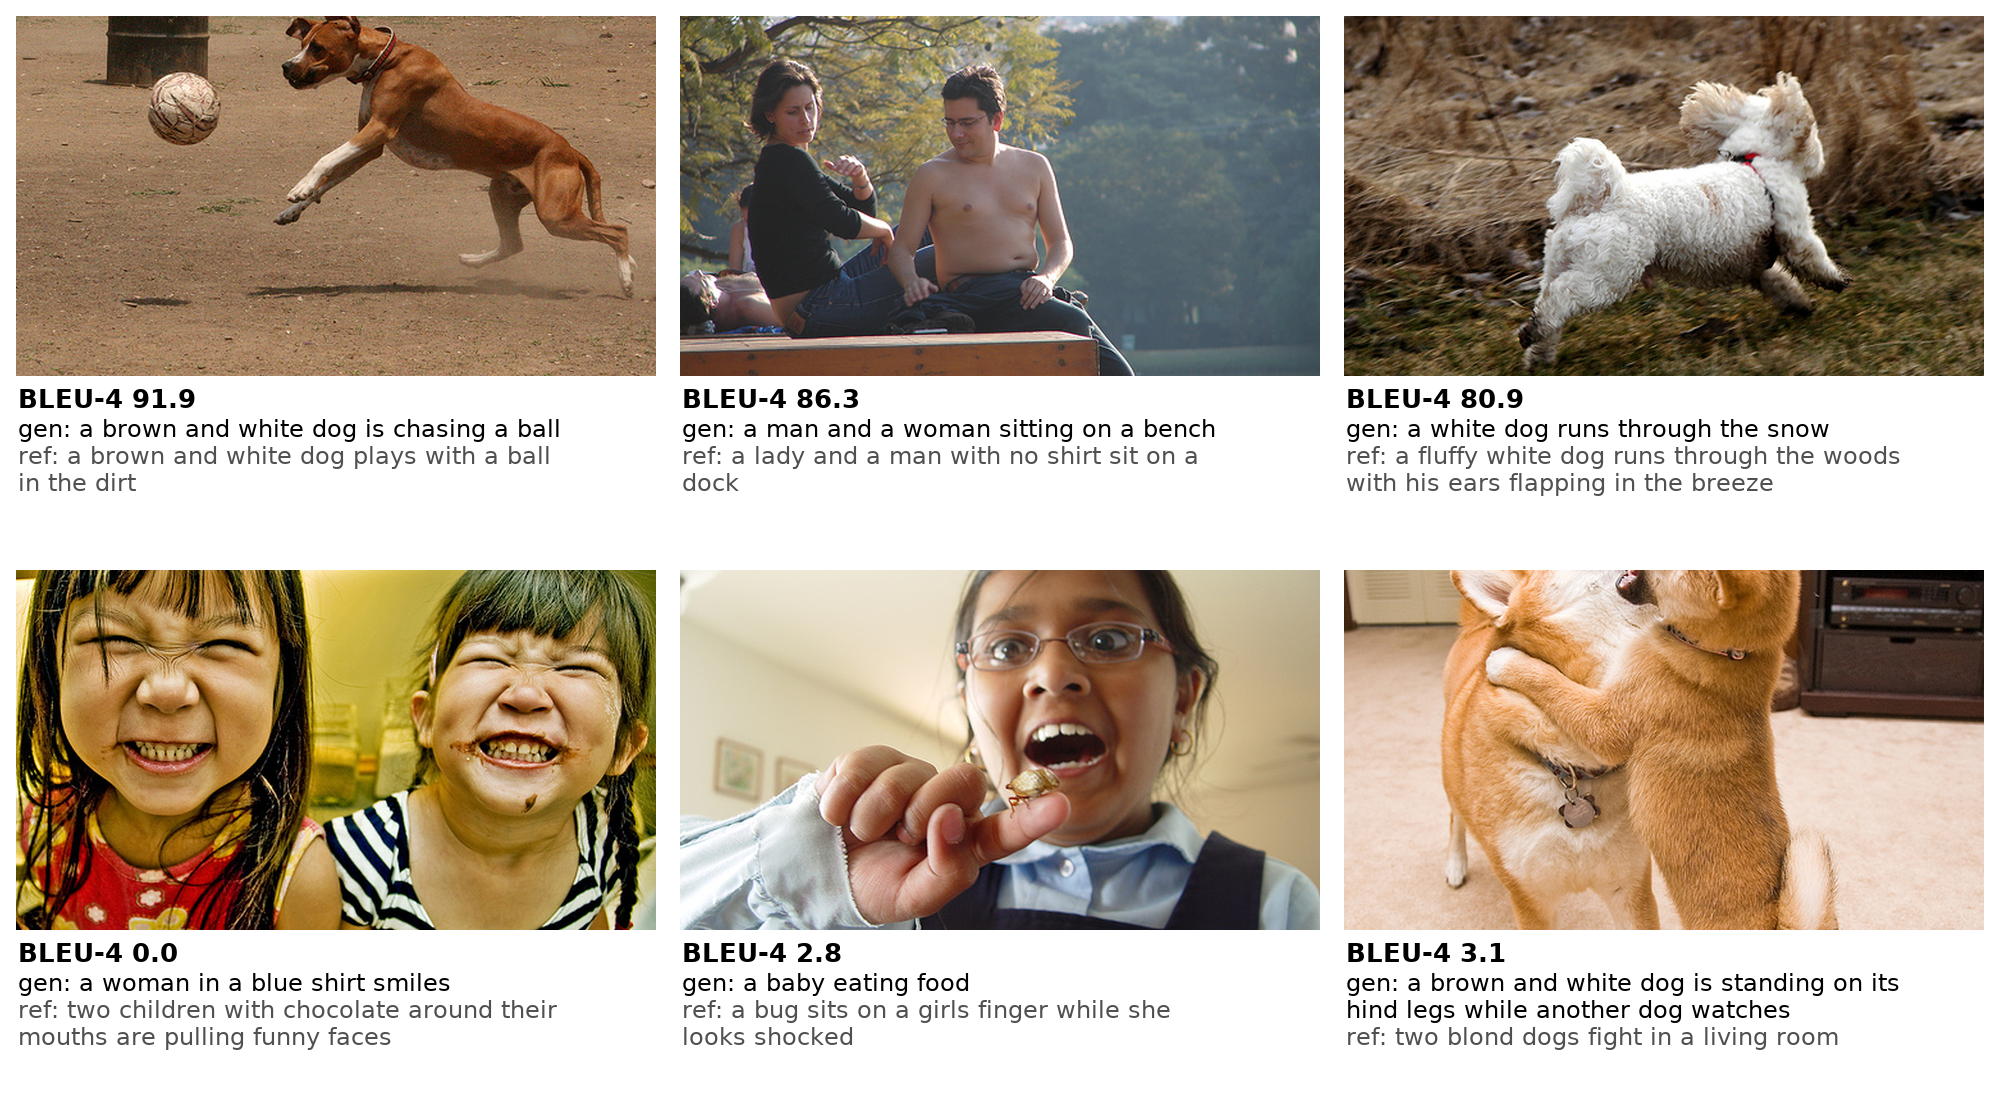
\includegraphics[width=0.9\textwidth]{../figures/fig5_examples_report.png}
\caption{Test examples from ResNet-50 with beam $k=5$: three high-scoring
captions (top) and three low-scoring ones (bottom), with one reference each.
The failures are semantic, not grammatical: children are called a woman, a
child eating is called a baby, and two playing dogs are given the wrong action.}
\label{fig:examples}
\end{figure*}

\subsection{Analysis}
\paragraph{Beam search versus greedy decoding}
Beam search buys about two BLEU-4 points for five times the decoding cost.
Widening the beam helps ResNet-50 (+0.37 from $k=3$ to $k=5$) but not
EfficientNet-B0 ($-0.03$): gains saturate once the top of the beam is decided by
the language model. Beam captions are 1.5 words shorter than greedy ones (9.16
versus 10.62; references 10.83). Because BLEU is precision-weighted, part of the
gain is brevity --- fewer, safer n-grams. Greedy output is more diverse (445
versus 405 distinct words), repeating generic words in longer captions.

\paragraph{Encoder comparison}
The encoders are effectively tied under beam search (21.64 versus 21.47);
validation losses agree (2.686 versus 2.715), and 0.17 BLEU-4 is one or two
captions. EfficientNet-B0 featurises twice as fast with 0.4M fewer parameters,
so it suits a tight budget; ResNet-50 is marginally better. The gap is larger
under greedy decoding (19.51 versus 18.05), where early errors are not corrected.

\paragraph{Qualitative errors}
Figure~\ref{fig:examples} shows the best and worst sentence scores. High scorers
are short and concrete (``a man and a woman sitting on a bench''). Failures are
semantic, not syntactic: two children with chocolate are called ``a woman in a
blue shirt smiles'' (0.0), a girl eating becomes ``a baby eating food'', and two
playing dogs get the wrong action. Colours and counts are dropped, and unknown
tokens appear in greedy output. A merge decoder compresses the whole image into
one vector, so fine details are lost; exactly eight captions match a reference
word for word, showing how strongly the score depends on reference choice.

\paragraph{Limitations}
Flickr8k is small and clean, and BLEU is sensitive to wording. Encoders are
frozen, so they never adapt to captioning; attention or fine-tuning should
improve compositional captions. Beam scores are not length-normalised, no
diversity decoding was tried, and results come from one seed, one split and a
shared T4 GPU.

\begin{table}[t]
\centering
\caption{Flickr8k statistics and preprocessing.}
\label{tab:data}
\footnotesize
\setlength{\tabcolsep}{3pt}
\begin{tabular}{@{}ll@{}}
\toprule
Property & Value \\
\midrule
Images / captions & 8,091 / 40,455 (5 per image) \\
Train / validation / test images & 6,000 / 1,000 / 1,091 \\
Test captions / OOV tokens & 5,455 / 3.24\% \\
Vocabulary before / after & 7,439 / 2,557 (min.\ freq.\ 5) \\
Sequence length & 22 tokens (max) \\
Caption length & 10.83 words mean, 10 median \\
Encoder input & 256 resize, 224 centre crop \\
\bottomrule
\end{tabular}
\end{table}

\begin{table}[t]
\centering
\caption{Test-set captioning results (1,091 images, 5,455 references). Best BLEU in bold.}
\label{tab:bleu}
\footnotesize
\setlength{\tabcolsep}{2.6pt}
\begin{tabular}{@{}llccccc@{}}
\toprule
Encoder & Decoding & B-1 & B-4 & Distinct & Length & Sec. \\
\midrule
ResNet-50 & greedy & 59.60 & 19.51 & 445 & 10.62 & 1.1 \\
ResNet-50 & beam $k{=}3$ & 62.46 & 21.27 & 408 & 9.71 & 4.0 \\
ResNet-50 & beam $k{=}5$ & 62.86 & \textbf{21.64} & 405 & 9.16 & 5.9 \\
EfficientNet-B0 & greedy & 58.68 & 18.05 & 364 & 10.51 & 0.8 \\
EfficientNet-B0 & beam $k{=}3$ & 62.78 & 21.50 & 351 & 9.76 & 3.9 \\
EfficientNet-B0 & beam $k{=}5$ & \textbf{63.19} & 21.47 & 345 & 9.22 & 5.9 \\
\bottomrule
\end{tabular}
\end{table}

\section{Conclusion}
A frozen ResNet-50 with a merge LSTM and beam search reaches BLEU-4 21.64,
about two points above greedy; EfficientNet-B0 is within 0.17 and twice as fast
to featurise. Remaining errors are semantic, pointing to visual attention and
unfrozen encoders as next steps.

\section*{AI Use Disclosure}
I used opencode, an AI coding assistant, for notebook scaffolding, figure code
and a first draft of this report's LaTeX, which I edited. I ran the notebook on
Kaggle, verified every number against the executed outputs, and checked splits
and leakage controls myself. I take full responsibility for this work.

\begin{thebibliography}{1}
\raggedright
\bibitem{hodosh} M.~Hodosh, P.~Young and J.~Hockenmaier, ``Framing image
description as a ranking task: Data, models and evaluation metrics,''
\emph{Journal of Artificial Intelligence Research}, vol.~47, pp.~853--899, 2013.

\bibitem{resnet} K.~He, X.~Zhang, S.~Ren and J.~Sun, ``Deep residual learning
for image recognition,'' \emph{Proc. CVPR}, 2016.

\bibitem{effnet} M.~Tan and Q.~Le, ``EfficientNet: Rethinking model scaling for
convolutional neural networks,'' \emph{Proc. ICML}, 2019.

\bibitem{sacrebleu} M.~Post, ``A call for clarity in reporting BLEU scores,''
\emph{Proc. WMT}, 2018.
\end{thebibliography}

\end{document}
